
%
% template for Bachelor thesis
% LIACS
% January 7, 2019
%

\documentclass[12pt]{article}

% include some packages
\usepackage[left=2cm,right=2cm,top=2cm,bottom=3cm]{geometry}
\usepackage{graphicx}
\usepackage{tikz}
\usepackage{tikz-cd}
\usetikzlibrary{shapes,backgrounds,calc,arrows}
\usepackage{microtype}
\usepackage{amsmath}
\usepackage[utf8]{inputenc}
\usepackage{amsfonts}
\usepackage{amssymb}
\usepackage{amsthm}

\newtheorem{definition}{Definition}[section]
\newtheorem{lemma}{Lemma}[section]

\usepackage{bbm}
\usepackage{geometry}
\usepackage{csquotes}
\usepackage[hidelinks]{hyperref}
\usepackage{mathtools}
\usepackage{parskip}

\usepackage{mathtools}
\newcommand{\defeq}{\vcentcolon=}
\newcommand{\eqdef}{=\vcentcolon}

\DeclareMathOperator{\Ima}{Im}
\DeclareMathOperator{\sech}{sech}
\renewcommand{\P}{\mathcal{P}}
\newcommand{\R}{\mathbb{R}}
\newcommand{\C}{\mathbb{C}}
\newcommand{\N}{\mathbb{N}}
\newcommand{\E}[1]{\mathbb{E}\{#1\}}
\newcommand{\Q}{\mathbb Q}
\newcommand{\Z}{\mathbb{Z}}
\newcommand{\1}{\mathbbm{1}}
\newcommand{\ua}{\nearrow}
\newcommand{\da}{\searrow}
\newcommand{\eps}{\varepsilon}
\newcommand{\dx}{\mathrm{d}x}
\newcommand{\B}{\mathcal{B}}
\newcommand{\F}{\mathcal{F}}
\newcommand{\T}{\mathbb{T}}
\newcommand{\V}{\mathcal{V}}
\newcommand{\U}{\mathcal{U}}
\newcommand{\id}{\text{id}}
\newcommand{\I}{\mathcal{I}}
\newcommand{\A}{\mathcal{A}}
\newcommand{\J}{\mathcal{J}}
\newcommand{\G}{\mathcal{G}}
\renewcommand{\L}{\mathcal{L}}
\newcommand{\specepsilon}{\mathcal{E}}
\newcommand{\M}{\mathcal{M}}
\newcommand{\II}{\textbf{II}}
\newcommand{\bigo}{\mathcal{O}}
\renewcommand{\H}{\mathcal{H}}
\usepackage[setpagesize=false,colorlinks=true,linkcolor=blue,urlcolor=red,pdftitle={An Interesting Title for a Thesis},pdfauthor={Your Name}]{hyperref}
\setlength\parindent{0pt}

\begin{document}
\thispagestyle{empty}


\includegraphics{logoleiden}

\vspace{-2.5cm}\hfill \begin{huge}\textbf{Opleiding Informatica}\end{huge}

\vspace{5cm}
\begin{Large}
\hfill Simplicial Coalgebras

\vspace*{3mm}

\hfill for Concurrent Regular Languages

\vspace*{14mm}

\hfill Hessel Sieburgh
\end{Large}

\vspace*{6.0cm}

\begin{large}

Supervisors:\\
Henning Basold \& 
Marton Hablicsek


\vspace*{2.8cm}
BACHELOR THESIS

\vspace*{5mm}
Leiden Institute of Advanced Computer Science (LIACS)\\
\href{www.liacs.leidenuniv.nl}{\underline{\texttt{www.liacs.leidenuniv.nl}}}\hfill 01/07/2025
\end{large}

\newpage



% abstract and references should fit on one page
\begin{abstract}
\noindent
This is where you write an abstract that concisely summarizes your thesis.
Keep it short. No references here --- exceptions do occur.
\end{abstract}

\bigskip

\thispagestyle{empty}
\tableofcontents
\thispagestyle{empty}
%Some (very few) people like a list of tables:
%\listoftables
%And some (even fewer) like a list of figures:
%\listoffigures

\clearpage
\setcounter{page}{1}

\section{Introduction} \label{introduction}

In this section we give an introduction to the problem addressed in this thesis.


\subsection{The situation}

Sections may include subsections.

To make sure that this document renders correctly, execute these commands:
\begin{quote}
\begin{verbatim}
pdflatex thesis
bibtex thesis
pdflatex thesis
pdflatex thesis
\end{verbatim}
\end{quote}
Here, the \verb|pdflatex| command may need to be executed three times in order to generate the table of contents and so on. 
Note that a good thesis has figures and tables; examples can be found in Figure~\ref{afigure} and Table~\ref{atable}. And every thesis has references, like~\cite{whatagreatpaper}.

\begin{figure}[!htbp]
\begin{center}
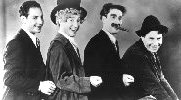
\includegraphics[height=2cm]{marxbrothers2}
\end{center}
\caption{Every thesis should have figures. Source: \href{www.marxbrothers.org}{\underline{\texttt{www.marxbrothers.org}}}.}\label{afigure}
\end{figure}

\begin{table}[!htbp]
\begin{center}
\begin{tabular}{l|l}
Column A & Column B\\
\hline
Point 1 & Good\\
Point 2 & Bad
\end{tabular}
\end{center}
\caption{Every thesis should have tables.}\label{atable}
\end{table}

Final reminder: this template is just an example, if you want you can make adjustments; also discuss with your supervisor which layout he or she likes. But the front page should be as it is now.

TODO: quite a lot!

\subsection{Thesis overview}
It is recommended to end the introduction with an overview of the thesis. This chapter contains the introduction; Section~\ref{definitions} includes the definitions; Section~\ref{relatedwork} discusses related work; Section~\ref{experiments} describes the experiments and their outcome; Section~\ref{conclusions} concludes. By the way, different section titles are certainly possible.

Also, produce a nice sentence with ``bachelor thesis'', LIACS and the names of the supervisors.
\section{Ranked Term Graphs}

\subsection{Definition and Structure}
\begin{definition}
    A directed \emph{hypergraph} $(V,H)$ is a set of vertices $V$ and a set of \emph{hyperarcs} $H\subseteq \P(V)^2$.
\end{definition}

\emph{Notation:} A directed hypergraph containing no cycles is a Directed Acyclic Hypergraph (DAH)\\

\begin{definition}
A \emph{ranked term hypergraph} $(g, r, o, \L, A)$ consists of:
\begin{itemize}
\item A DAH $g$,
\item Sequences $r = (r_i)_{i\in[|r|]}$, $o = (o_i)_{i\in[|o|]}$ $r_i, o_i\in \P(V)$ denoting the root and variable interfaces. $o_i$ contains only maximal vertices. We refer to $(|r|, |o|)$ as the \emph{rank} of this graph.
\item An action set $A$ and a hyperarc labelling function $\L: H\to A$
\end{itemize}
\end{definition}
\emph{Notation:} In this thesis we refer to ranked term hypergraphs as just hypergraphs as we will only be working with this kind. $HG(n,m)$ is the set of ranked term  hypergraphs of rank $(n,m)$

A ranked hypergraph with $|r| = |o|$ is called symmetric.

\subsection{Composition of ranked hypergraphs}
\begin{definition}
Let $G, F$ be hypergraphs such that $|o^G| = |r^F|$, their composition is defined as follows:
\begin{align}
    G\circ F = (g', r', o^F, L^G\cup L^F, A^G\cup A^F)
\end{align}

We obtain $g'$ by the following procedure:
\begin{enumerate}
    \item $g' = (V,H) \defeq g^G \sqcup g^F$
    \item For each $o^G_i\in o^G$, $v\in o^G_i$: $V\defeq V\setminus \{v\}$ and for each $(U, U')\in H$ with $v\in U'$ set $U' \defeq (U' \cup r^F_i) \setminus \{v\}$\\
\end{enumerate}

And we obtain $r'$ by taking over the original $r^G$ and `connecting through' for vertices which are both minimal and maximal:
\begin{align*}
    r'_i = \{v\in r_i^G: v \text{ is not maximal}\}\cup \{v\in r_j^F : r^G_i \cap o_j^F \neq \varnothing,  j\in[|r^F|]\}
   %  \begin{cases} 
   %     \{v\in r_i^G: v \text{ is not maximal}\}& o _i^G \text{ contains at least 1 non-maximal vertex} \\
   %     r_i^F & \text{else}
   % \end{cases}
\end{align*}
\end{definition}

This composition allows for an identity $id_n$ namely $id_n = (([n], \varnothing), (\{i\})_{i\in n}, (\{i\})_{i\in n})$. It holds clearly from the definition that for a $(n,m)$ ranked graph $G$ holds: $$id_n \circ G = G \circ id_m = G$$
\newpage
\section{Simplicial set over ranked term graphs}
\subsection{Monoidal structure on interfaces}
\begin{definition}
    Let $V$ be the vertex set of a ranked hypergraph.\\
    We define the monoid $\M = (\P(V)^2, (\varnothing, \varnothing), \cup\times\cup)$. 
\end{definition}

From this monoid we define a simplicial set using the nerve construction.

\begin{definition}
    The \emph{nerve} $N(\M)$ of the monoid $\M$ is the simplicial set where:
    \begin{align*}
        &N(\M)_n = \M^n\\
        &d_i(m_1,\dots,m_n) = 
        \begin{cases}
            (m_1,\dots,m_i \cup\times\cup m_{i+1}, \dots, m_n) & 0 < i < n\\
            (m_2,\dots, m_n) & i = 0\\
            (m_1,\dots,m_{n-1}) & i = n
        \end{cases}\\
        &s_i(m_1,\dots,m_n) = (m_1, \dots, m_i, (\varnothing, \varnothing), m_{i+1}, \dots, m_n)\\
    \end{align*}
\end{definition}

\begin{definition}
Define the simplicial set $\H$ by $\H_n = HG(n,n)$. The face and degeneracy maps of $\H$ are defined to be the unique maps $d^{\H}$, $s^{\H}$ making the following diagrams commute:
\[
\begin{tikzcd}
\H_n \arrow{r}{d_i^{\H}} \arrow{d}{\pi_n} & \H_{n-1} \arrow{d}{\pi_{n-1}} \\
N(\M)_n \arrow{r}{d_i^\M} & N(\M)_{n-1}
\end{tikzcd}
\quad
\begin{tikzcd}
\H_n \arrow{r}{s_j^{\H}} \arrow{d}{\pi_n} & \H_{n+1} \arrow{d}{\pi_{n+1}} \\
N(\M)_n \arrow{r}{s_j^\M} & N(\M)_{n+1}
\end{tikzcd}
\]

Where $\pi_n$ is the projection onto the interfaces given by: $\pi_n((g, r, o, \L, A)) = ((r_i, o_i))_{i\in [n]}$. That is, the face and degeneracy maps of $\H$ are defined by the underlying monoidal nerve on the interfaces.
\end{definition}

$\H$ is a simplicial set precisely because we inherit the face and degeneracy maps from $N(\M)$:\\

\begin{lemma}
    $\H$ is indeed a simplicial set.
\end{lemma}

\begin{proof}
    $\pi_n$ is a simplicial morphism by commutation of the given diagrams. Since $N(\M)$ is a simplicial set by definition and the diagrams commute the simplicial identities also hold for $d^{\H}$ and $s^{\H}$. Therefore $\H$ is a simplicial set.
\end{proof}

\newpage
\section{Related Work}\label{relatedwork}

\section{Experiments}\label{experiments}

\section{Conclusions and Further Research}\label{conclusions}

\bibliographystyle{alpha}
\bibliography{bibliography}
\addcontentsline{toc}{section}{References}


%\appendix
%appendices here --- if any

\end{document}